\documentclass{standalonex}
\usepackage{tikz}

\begin{document}
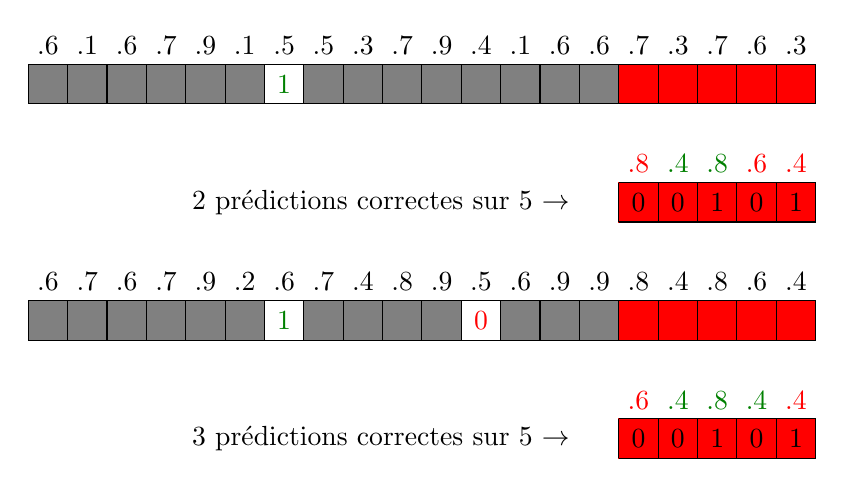
\begin{tikzpicture}[scale=0.5]
\filldraw[black!50] (0,0) rectangle (6,1);
\filldraw[black!50] (7,0) rectangle (15,1);
\filldraw[red] (15,0) rectangle (20,1);
\draw (0,0) grid (20,1);
\node[green!50!black] at (6.5,0.5) {1};
\node[above] at (0.5,1) {.6};
\node[above] at (1.5,1) {.1};
\node[above] at (2.5,1) {.6};
\node[above] at (3.5,1) {.7};
\node[above] at (4.5,1) {.9};
\node[above] at (5.5,1) {.1};
\node[above] at (6.5,1) {.5};
\node[above] at (7.5,1) {.5};
\node[above] at (8.5,1) {.3};
\node[above] at (9.5,1) {.7};
\node[above] at (10.5,1) {.9};
\node[above] at (11.5,1) {.4};
\node[above] at (12.5,1) {.1};
\node[above] at (13.5,1) {.6};
\node[above] at (14.5,1) {.6};
\node[above] at (15.5,1) {.7};
\node[above] at (16.5,1) {.3};
\node[above] at (17.5,1) {.7};
\node[above] at (18.5,1) {.6};
\node[above] at (19.5,1) {.3};
\begin{scope}[yshift=-3cm]
    \filldraw[red] (15,0) rectangle (20,1);
    \draw (15,0) grid (20,1);
    \node[above,red] at (15.5,1) {.8};
    \node[above,green!50!black] at (16.5,1) {.4};
    \node[above,green!50!black] at (17.5,1) {.8};
    \node[above,red] at (18.5,1) {.6};
    \node[above,red] at (19.5,1) {.4};
    \node at (15.5,0.5) {0};
    \node at (16.5,0.5) {0};
    \node at (17.5,0.5) {1};
    \node at (18.5,0.5) {0};
    \node at (19.5,0.5) {1};
    \node[left] at (14,0.5) {2 prédictions correctes sur 5 $\rightarrow$};
\end{scope}
\begin{scope}[yshift=-6cm]
    \filldraw[black!50] (0,0) rectangle (6,1);
    \filldraw[black!50] (7,0) rectangle (11,1);
    \filldraw[black!50] (12,0) rectangle (15,1);
    \filldraw[red] (15,0) rectangle (20,1);
    \draw (0,0) grid (20,1);
    \node[green!50!black] at (6.5,0.5) {1};
    \node[red] at (11.5,0.5) {0};
    \node[above] at (0.5,1) {.6};
    \node[above] at (1.5,1) {.7};
    \node[above] at (2.5,1) {.6};
    \node[above] at (3.5,1) {.7};
    \node[above] at (4.5,1) {.9};
    \node[above] at (5.5,1) {.2};
    \node[above] at (6.5,1) {.6};
    \node[above] at (7.5,1) {.7};
    \node[above] at (8.5,1) {.4};
    \node[above] at (9.5,1) {.8};
    \node[above] at (10.5,1) {.9};
    \node[above] at (11.5,1) {.5};
    \node[above] at (12.5,1) {.6};
    \node[above] at (13.5,1) {.9};
    \node[above] at (14.5,1) {.9};
    \node[above] at (15.5,1) {.8};
    \node[above] at (16.5,1) {.4};
    \node[above] at (17.5,1) {.8};
    \node[above] at (18.5,1) {.6};
    \node[above] at (19.5,1) {.4};
\end{scope}
\begin{scope}[yshift=-9cm]
    \filldraw[red] (15,0) rectangle (20,1);
    \draw (15,0) grid (20,1);
    \node[above,red] at (15.5,1) {.6};
    \node[above,green!50!black] at (16.5,1) {.4};
    \node[above,green!50!black] at (17.5,1) {.8};
    \node[above,green!50!black] at (18.5,1) {.4};
    \node[above,red] at (19.5,1) {.4};
    \node at (15.5,0.5) {0};
    \node at (16.5,0.5) {0};
    \node at (17.5,0.5) {1};
    \node at (18.5,0.5) {0};
    \node at (19.5,0.5) {1};
    \node[left] at (14,0.5) {3 prédictions correctes sur 5 $\rightarrow$};
\end{scope}
\end{tikzpicture}
\end{document}
